\section{Analyses}
\label{sec:analyses}

% Interprétation des résultats et comparaison avec les valeurs du constructeur.

% =====================================================================
% Chapitres 6 à 9 du rapport « Banc d'essai cogénération »
% À coller à la place des sections vides « Analyses », « Avantages »,
% « Inconvénients » et « Conclusion ».
%
% Paquets nécessaires : amsmath, graphicx, booktabs (+ url/hyperref
% pour la bibliographie). Les figures sont dans le dossier
% figures_analyse/ (à copier à côté du fichier .tex principal).
% Les références existantes [1] à [7] sont écrites en dur ; les
% nouvelles références (\cite{...}) sont à ajouter à la bibliographie
% (voir le bloc commenté à la fin de ce fichier).
% =====================================================================

Ce chapitre interprète les résultats du chapitre~5 et les compare aux
valeurs du constructeur (tableau~1). Sauf mention contraire, les
grandeurs sont calculées sur l'ensemble de l'essai (115~min), à partir
des variations d'index des compteurs et de la puissance thermique
fournie par le programme d'acquisition.

\subsection{Méthode : énergies cumulées plutôt que valeurs instantanées}
\label{sec:methode}

Les rendements du tableau~4 sont des moyennes de rapports calculés tous
les 5~minutes. Or ces rapports fluctuent fortement : le rendement global
instantané varie de 55,4 à 83,0~\%, alors que la puissance thermique
est quasi constante (de 8,3 à 10,4~kW). Cette dispersion vient du
fait que la puissance du gaz consommé varie de
17,4 à 26,5~kW alors qu'un moteur à régime stable ne devrait pas présenter de
telles variations. Chaque pas de 5~minutes ne correspond qu'à environ
0,2~m$^3$ de gaz : une incertitude d'une minute sur l'instant de lecture
du compteur manuel suffit à modifier la puissance de $\pm 20$~\%. Les
valeurs instantanées, y compris le maximum de 83~\% à 70~min, sont donc
des erreurs de mesure et non un fonctionnement réel proche des 85~\%
du constructeur.

Afin de s'affranchir de ce bruit, nous travaillons sur les énergies
cumulées sur la durée de l'essai :
\begin{equation}
  \eta_{\mathrm{el}} = \frac{E_{\mathrm{el}}}{E_{\mathrm{gaz}}},
  \qquad
  \eta_{\mathrm{th}} = \frac{Q_{\mathrm{th}}}{E_{\mathrm{gaz}}},
  \qquad
  \eta_{\mathrm{global}} = \eta_{\mathrm{el}} + \eta_{\mathrm{th}}
  \label{eq:rendements_cumules}
\end{equation}
avec $E_{\mathrm{gaz}} = \Delta V \cdot \rho \cdot \mathrm{PCI}/3{,}6$
(en kWh, avec $\rho \cdot \mathrm{PCI} = 35$~MJ/m$^3$),
$E_{\mathrm{el}}$ la variation d'index du compteur d'électricité et
$Q_{\mathrm{th}} = \sum_i P_{\mathrm{th},i} \cdot 5/60$ la chaleur
récupérée. Sur 115~minutes, la cogénération a consommé 43,2~kWh de gaz
(4,442~m$^3$), produit 10,59~kWh d'électricité et récupéré 17,7~kWh de
chaleur, soit :
\begin{equation}
  \eta_{\mathrm{el}} = 24{,}5~\%, \qquad
  \eta_{\mathrm{th}} = 41{,}0~\%, \qquad
  \eta_{\mathrm{global}} = 65{,}5~\%
\end{equation}
Ces valeurs sont proches des moyennes du tableau~4 (24,7~\%, 41,8~\%
et 66,4~\%), mais elles sont moins sensibles aux erreurs de lecture.
La figure~\ref{fig:cumul} montre que les trois énergies cumulées évoluent
linéairement avec le temps, ce qui confirme un régime stable dès les
premières minutes.

\begin{figure}[htbp]
  \centering
  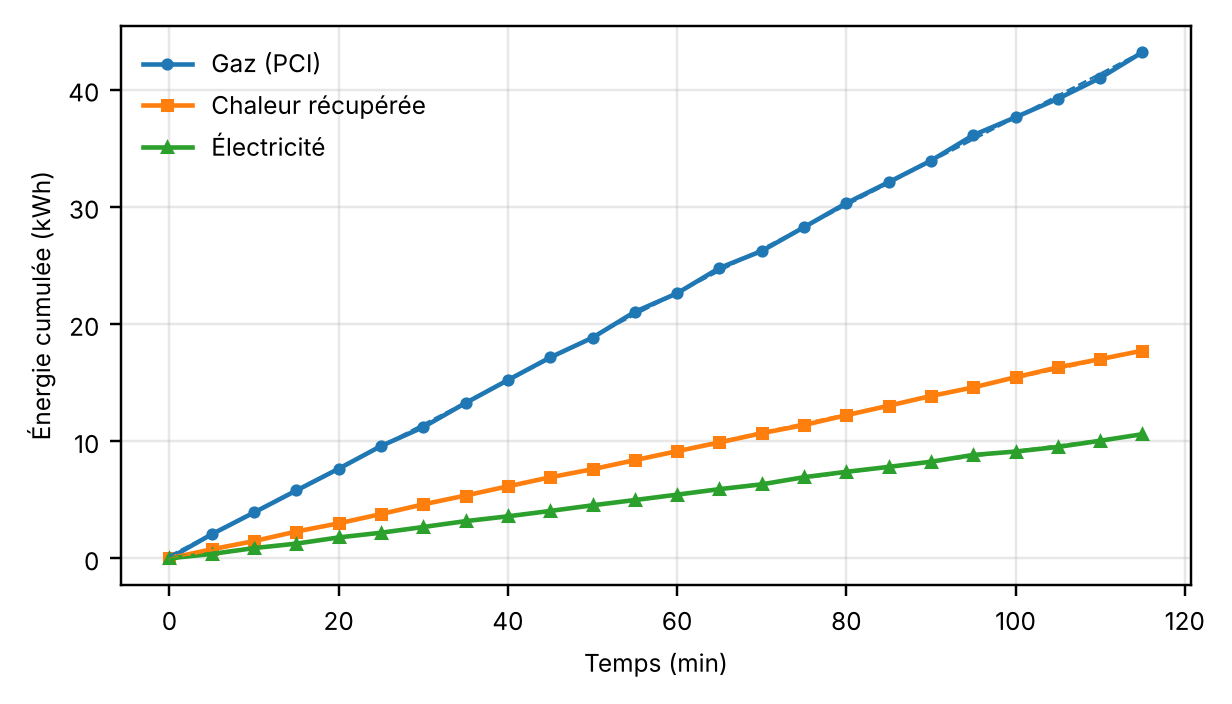
\includegraphics[width=0.9\textwidth]{figures_analyse/fig_energies_cumulees.png}
  \caption{Énergies cumulées (gaz, chaleur récupérée, électricité)}
  \label{fig:cumul}
\end{figure}

\subsection{Comparaison avec les valeurs du constructeur}
\label{sec:comparaison}

Le tableau~\ref{tab:comparaison} compare les valeurs mesurées à celles
du constructeur (tableau~1).

\begin{table}[htbp]
  \centering
  \caption{Valeurs mesurées (énergies cumulées sur 115~min) et valeurs du constructeur}
  \label{tab:comparaison}
  \begin{tabular}{lccc}
    \toprule
    Grandeur & Constructeur & Mesuré & Écart \\
    \midrule
    Puissance du gaz (kW)          & 20,8 & 22,5 & $+8$~\% \\
    Puissance électrique (kW)      & 6,0  & 5,5  & $-8$~\% \\
    Puissance thermique (kW)       & 11,7 & 9,2  & $-21$~\% \\
    Rendement électrique (\%)      & 28,8 & 24,5 & $-4{,}3$ points \\
    Rendement thermique (\%)       & 56,2 & 41,0 & $-15{,}2$ points \\
    Rendement global (\%)          & 85,0 & 65,5 & $-19{,}5$ points \\
    \bottomrule
  \end{tabular}
\end{table}

Le rendement global mesuré est inférieur de près de 20 points à celui du
constructeur. Cet écart se répartit entre une baisse de 4,3~points sur
le rendement électrique et de 15,2~points sur le rendement thermique.
Plusieurs éléments permettent de nuancer ou d'expliquer ces écarts.

\paragraph{Puissance du gaz.} La puissance du gaz dépend du produit
$\rho \cdot \mathrm{PCI}$ supposé, qui est une valeur générique, et du
volume lu au compteur, qui n'est pas corrigé en pression et en
température. Le pouvoir calorifique réel du gaz distribué (indiqué par
le gestionnaire de réseau ou sur une facture) peut s'écarter de
quelques pour cent de notre hypothèse. La valeur du constructeur est donnée dans des conditions de
référence (100~kPa, 25~°C, 30~\% d'humidité) et la base de calcul
(PCI ou PCS) n'est pas précisée dans [3] ; elle devrait être vérifiée,
car un rendement exprimé sur PCS serait inférieur d'environ 10~\% à un
rendement exprimé sur PCI.

\paragraph{Puissance électrique.} La puissance électrique de sortie
(\emph{W out}) affichée par le logiciel d'acquisition reste exactement à 6\,000~W à chaque
relevé : une valeur aussi constante est probablement une consigne ou une
valeur nominale affichée plutôt qu'une mesure. À 6~kW, l'unité aurait
produit 11,5~kWh en 115~min, contre 10,59~kWh lus au compteur
(soit $-8$~\%). Nous retenons donc la valeur du
compteur (5,5~kW en moyenne), plus fiable. Elle est plus cohérente, notamment avec le
premier pas de 5~min qui a une moyenne 4,4~kW, ce qui correspondrait à la montée en puissance
au démarrage.

\paragraph{Puissance thermique.} La puissance thermique récupérée
(9,2~kW) est inférieure de 21~\% à celle du constructeur. L'écart ne
s'explique pas par la température d'entrée de l'eau : le constructeur
raisonne avec un retour à 60~°C, alors que celui de notre essai se situe
entre 20 et 49~°C, ce qui favorise plutôt l'échange avec le liquide de
refroidissement. Le débit n'a pas été mesuré, mais il peut être estimé à
partir de l'écart de température entre l'entrée et la sortie du ballon
(7,9 à 11,1~°C, moyenne de 9,6~°C) :
\begin{equation}
  \dot{m} = \frac{P_{\mathrm{th}}}{c_p \,\Delta T}
  \approx \frac{9{,}2}{4{,}186 \times 9{,}6} \approx 0{,}23~\mathrm{kg/s}
  \approx 14~\mathrm{L/min}
\end{equation}
Cette estimation (de 11 à 17~L/min selon le relevé) suppose que la
puissance thermique de l'acquisition est correcte ; elle ne peut donc
pas la valider. Elle indique toutefois que le débit réel était nettement
inférieur aux 34,1~L/min du constructeur : avec 34,1~L/min et un écart
de 9,6~K, la puissance serait de 22~kW, soit toute la puissance du gaz
consommé, ce qui est impossible. Notre essai ne s'est donc déroulé ni
au débit ni à la température de retour de référence, et les écarts du
tableau~\ref{tab:comparaison} ne sont pas comparables au
point de fonctionnement du constructeur. Pour une exploitation correcte,
il faudrait mesurer le débit d'eau sortant de la machine lors
d'un prochain essai.

\subsection{Bilan énergétique et pertes}
\label{sec:bilan}

La figure~\ref{fig:bilan} compare la répartition de l'énergie du gaz (énergie consommée)
selon le constructeur et selon notre essai. Les pertes passent de
15,0~\% à 34,5~\%.

\begin{figure}[htbp]
  \centering
  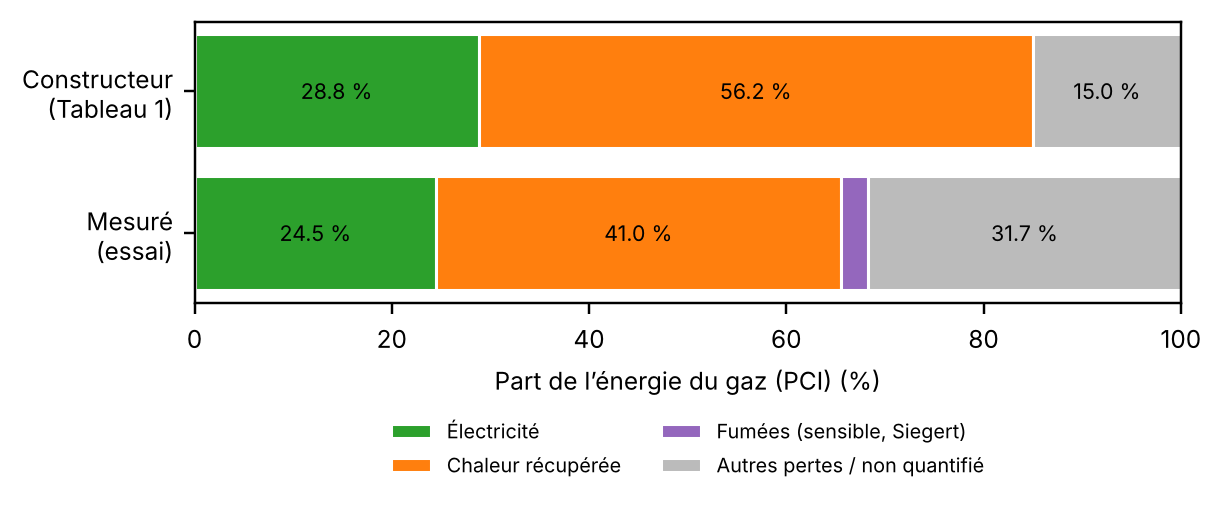
\includegraphics[width=0.9\textwidth]{figures_analyse/fig_bilan_energetique.png}
  \caption{Répartition de l'énergie du gaz (base PCI) : valeurs du
  constructeur et valeurs mesurées}
  \label{fig:bilan}
\end{figure}

Parmi ces pertes, nous pouvons en quantifier deux à partir de
l'analyseur de combustion :
\begin{itemize}
  \item \emph{la chaleur sensible des fumées}, par la formule de
  Siegert $q_A = (T_{\mathrm{fum}} - T_{\mathrm{amb}}) \left(\frac{A_2}{21 - \mathrm{O}_2} + B\right)$,
  avec les coefficients usuels du gaz naturel ($A_2 = 0{,}66$ et
  $B = 0{,}009$). Avec un écart de température de 45~°C environ et
  8,8~\% d'O$_2$, on obtient $q_A \approx 2{,}8$~\% (0,64~kW) ;
  \item \emph{le CO imbrûlé}, dont la combustion libérerait environ
  0,2~\% de l'énergie du gaz (calcul à partir du rapport
  $\mathrm{CO}/(\mathrm{CO} + \mathrm{CO}_2)$ et des pouvoirs
  calorifiques du CO et du méthane).
\end{itemize}
Ces deux postes ne représentent que 3~\% de l'énergie du gaz : les
fumées ne sont donc pas la cause principale de l'écart. Il reste
environ 31,5~\% d'énergie non expliquée, contre 15~\% pour le
constructeur. Elle regroupe plusieurs postes que nos mesures ne
permettent pas de séparer : les pertes du générateur et de l'onduleur,
la chaleur cédée à l'air de l'armoire par le moteur et le circuit de
refroidissement, un
éventuel passage dans le radiateur interne (section~2.2), les
hydrocarbures imbrûlés d'un moteur à mélange pauvre (non mesurés), et
enfin les erreurs sur le pouvoir calorifique et sur la puissance
thermique de l'acquisition.

\subsection{Circuit hydraulique et radiateurs}
\label{sec:hydraulique}

\paragraph{Vitesse d'échauffement.} Les pentes de température du ballon
sont reprises dans le tableau~\ref{tab:pentes}. Elles diminuent au fur
et à mesure que l'essai avance, alors que la puissance thermique reste
constante : l'ouverture des radiateurs (à partir de 65~min) et les
pertes thermiques croissantes de la cuve absorbent une part de plus en
plus grande de la chaleur.

\begin{table}[htbp]
  \centering
  \caption{Vitesse d'échauffement de l'eau du ballon (K/min)}
  \label{tab:pentes}
  \begin{tabular}{lccc}
    \toprule
    Fenêtre (min) & Entrée du ballon & Sortie du ballon (retour) & Radiateurs \\
    \midrule
    30 à 60  & 0,34 & 0,36 & fermés \\
    60 à 90  & 0,27 & 0,29 & ouverts \\
    90 à 115 & 0,15 & 0,17 & ouverts puis fermés \\
    \bottomrule
  \end{tabular}
\end{table}

\paragraph{Capacité thermique équivalente et bilan de chaleur.}
Entre 30 et 60~min, les radiateurs sont fermés et la quasi-totalité de
la chaleur récupérée (9,1~kW en moyenne) sert à chauffer l'eau, dont la
température moyenne (moyenne de l'entrée et de la sortie du ballon)
augmente de 0,41~K/min. On en déduit une capacité thermique équivalente
d'environ 1\,340~kJ/K, soit l'équivalent de 320~kg d'eau. Une seconde
estimation est possible : le front d'eau froide atteint la sortie du
ballon vers 27~min ; à un débit de 14~L/min, cela correspond à un
volume d'environ 380~L. Les deux ordres de grandeur sont cohérents
(300 à 400~L) et sont à comparer au volume réel de la cuve, qui n'a pas
été relevé.

En conservant cette capacité thermique, on estime la part de chaleur
qui n'est pas stockée (tableau~\ref{tab:bilan_cuve}). Elle correspond à
la chaleur dissipée par les radiateurs et par les pertes de la cuve.

\begin{table}[htbp]
  \centering
  \caption{Bilan de chaleur de la cuve (estimation)}
  \label{tab:bilan_cuve}
  \begin{tabular}{lccc}
    \toprule
    Fenêtre (min) & $P_{\mathrm{th}}$ (kW) & Stockée (kW) & Radiateurs et pertes (kW) \\
    \midrule
    60 à 90  & 9,4 & 6,1 & 3,3 \\
    90 à 115 & 9,3 & 4,0 & 5,3 \\
    \bottomrule
  \end{tabular}
\end{table}

Sur l'ensemble de la période de 30 à 115~min, environ 70~\% de la
chaleur récupérée (9,2 sur 13,1~kWh) est stockée dans l'eau, et 30~\%
est dissipée. Pour comparer, si tout le débit estimé (0,23~kg/s)
traversait le grand radiateur, son écart de température de 2,2 à 4,8~K
correspondrait à une puissance de 2,1 à 4,6~kW, ce qui est du même ordre
de grandeur que les valeurs du tableau~\ref{tab:bilan_cuve}. Ce bilan
reste toutefois une estimation, car il repose sur un débit non mesuré
et sur des sondes dont la précision est de $\pm 1{,}3$~K.

\subsection{Composition des fumées}
\label{sec:fumees}

\paragraph{Excès d'air.} À partir de la teneur en O$_2$, le coefficient
d'excès d'air $\lambda = 21/(21 - \mathrm{O}_2)$ vaut 1,74 en moyenne
(de 1,62 à 2,12). Le moteur fonctionne donc bien en mélange pauvre,
comme annoncé à la section~3.1.

\paragraph{Vérification du CO$_2$.} L'analyseur ne mesure pas le CO$_2$ :
il le calcule à partir de l'O$_2$ et du CO$_2$ maximal du combustible
sélectionné. Les valeurs de l'annexe (8,42~\% pour 8,0~\% d'O$_2$)
correspondent à un CO$_2$ maximal d'environ 13,6~\%, alors qu'il vaut
environ 11,9~\% pour le gaz naturel. Avec cette dernière valeur, le CO$_2$
serait de 6,9~\% en moyenne (de 5,6 à 7,4~\%) au lieu de 7,9~\%. Il est
donc probable que l'analyseur n'était pas réglé sur le gaz naturel. Cela
n'affecte pas l'O$_2$ ni le CO, mesurés directement, mais le CO$_2$ que nous avons mesuré est très probablement faux.

\paragraph{Niveau de CO.} Le CO est compris entre 393 et 588~ppm (moyenne
de 486~ppm), soit un écart bien supérieur à la précision de l'appareil
($\pm 20$~ppm ou $\pm 5$~\%) : les variations sont réelles. Pour comparer
des mesures à des teneurs en O$_2$ différentes, on ramène le CO à une
teneur de référence :
\begin{equation}
  \mathrm{CO}_{\mathrm{ref}} = \mathrm{CO} \cdot \frac{21 - \mathrm{O}_{2,\mathrm{ref}}}{21 - \mathrm{O}_2}
\end{equation}
Ramené à 0~\% d'O$_2$, le CO vaut 842~ppm en moyenne (de 640 à 1\,100~ppm).
La figure~\ref{fig:co} montre que la baisse apparente du CO après
60~min (de 491 à 480~ppm en moyenne) accompagne la hausse de l'O$_2$ (de
8,1 à 9,7~\% en moyenne) : c'est un effet de dilution. Ramené à 0~\%
d'O$_2$, le CO augmente même de 798 à 890~ppm entre les deux périodes.
La combustion ne s'est donc pas améliorée. L'oscillation de l'O$_2$
après 60~min coïncide avec l'ouverture des radiateurs, mais nos mesures
ne permettent pas d'établir un lien.

\begin{figure}[htbp]
  \centering
  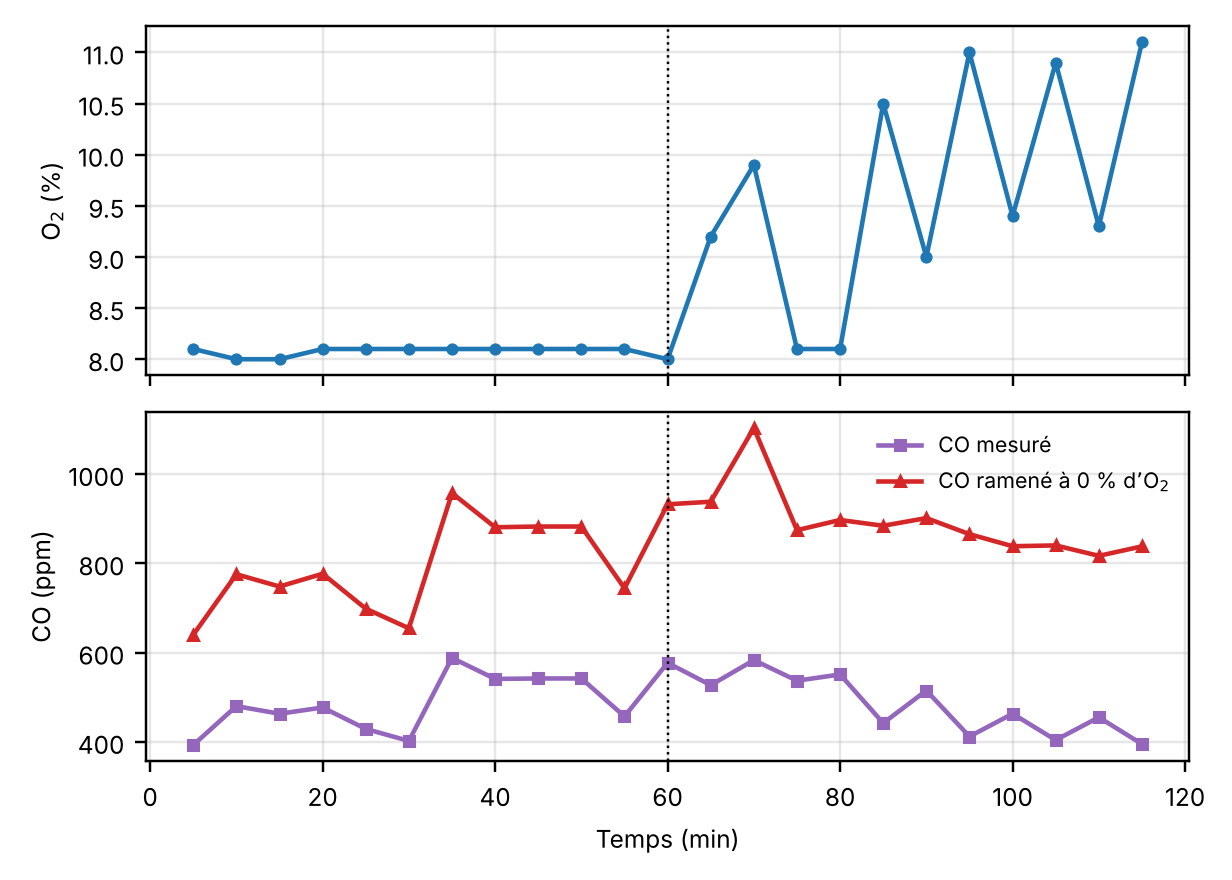
\includegraphics[width=0.85\textwidth]{figures_analyse/fig_co_normalise.png}
  \caption{Teneur en O$_2$ (haut), CO mesuré et CO ramené à 0~\% d'O$_2$
  (bas). La ligne en pointillés marque 60~min.}
  \label{fig:co}
\end{figure}

\paragraph{Repères sur les niveaux de CO.} Les seuils d'exposition
usuels (de l'ordre de 35~ppm sur 8~heures, 200~ppm sur 15~minutes et
1\,200~ppm pour un danger immédiat pour la vie [1]) sont largement
dépassés par les gaz d'échappement : l'évacuation des fumées vers
l'extérieur par la conduite de ventilation (figure~2) est donc
indispensable. Pour les émissions, la Région de Bruxelles-Capitale
impose aux moteurs au gaz naturel neufs de cogénération de 20~kW et plus
une valeur limite de 112,5~mg/Nm$^3$ de CO à 15~\% d'O$_2$
\cite{bxl_cogeneration}. Notre mesure convertie dans les mêmes
conditions (1~ppm de CO $=$ 1,25~mg/Nm$^3$) vaut environ 300~mg/Nm$^3$,
soit 2,7 fois cette limite (environ 800~mg/Nm$^3$ à 5~\% d'O$_2$). Cette
limite montre que la cogen de l'école n'est pas au
niveau des exigences actuelles. Nous n'avons pas mesuré les NO$_x$.

\subsection{Économie d'énergie primaire}
\label{sec:pes}

Pour juger l'intérêt énergétique d'une cogénération, on compare le gaz
consommé à celui qui serait nécessaire pour produire séparément la même
électricité (dans une centrale) et la même chaleur (dans une chaudière).
L'économie d'énergie primaire est
\begin{equation}
  \mathrm{PES} = 1 - \frac{1}{\dfrac{\eta_{\mathrm{th}}}{\eta_{\mathrm{ref,th}}} + \dfrac{\eta_{\mathrm{el}}}{\eta_{\mathrm{ref,el}}}}
  \label{eq:pes}
\end{equation}
Nous prenons pour le gaz naturel des rendements de référence de 52,5~\%
pour l'électricité et de 90~\% pour la chaleur, d'après le règlement
délégué (UE) 2015/2402 \cite{reglement_ref}. Les valeurs exactes
dépendent de l'année de construction de l'unité, et nous n'appliquons
pas le facteur de correction lié aux pertes de réseau évitées. Pour une
cogénération de moins de 1~MW électrique, la directive 2012/27/UE exige
une économie positive. Les résultats sont :
\begin{itemize}
  \item avec les valeurs du constructeur ($\eta_{\mathrm{el}} = 28{,}8$~\%
  et $\eta_{\mathrm{th}} = 56{,}2$~\%) : $\mathrm{PES} = +14{,}7$~\% ;
  \item avec nos valeurs mesurées ($\eta_{\mathrm{el}} = 24{,}5$~\%
  et $\eta_{\mathrm{th}} = 41{,}0$~\%) : $\mathrm{PES} = -8{,}4$~\%.
\end{itemize}
À performances mesurées, la cogénération consomme donc plus de gaz que
la production séparée. Pour atteindre une économie nulle avec notre
rendement électrique, il aurait fallu un rendement thermique d'au moins
48~\%. Ce résultat dépend du fonctionnement au point nominal, et il suppose
que toute la chaleur produite est utilisée.
